\section{Preprocessing}\label{s:preprocessing}

% Enumerated list
\begin{enumerate}
    \item Dropping non-relevant columns.
    \item Encoding the categorical target variable.
    \item Handling missing values using median imputation.
    \item Scaling numerical features to standardize the data.
    \item Combining all preprocessing steps using \texttt{ColumnTransformer}.
\end{enumerate}

\subsection{Data Encoding and Splitting}\label{ss:encoding}
The target variable \col{SpType-ELS}, a categorical variable, was encoded using \texttt{LabelEncoder} to convert
categorical values into a binary numerical format (\cref{lst:label_encoder}).

% Code listing with caption and label; styles: python, bash (see assignment.sty)
\begin{lstlisting}[style=python, caption={Encoding the target variable}, label={lst:label_encoder}]
from sklearn.preprocessing import LabelEncoder

label_encoder = LabelEncoder()
y_encoded = label_encoder.fit_transform(y)  # "A" -> 0, "B" -> 1
\end{lstlisting}

% Simple table with booktabs rules
\Cref{tab:classifiers} summarizes the classifiers used and maps them to the techniques discussed in class where
applicable.
\begin{table}[H]
    \centering
    \begin{tabular}{lll}
        \toprule
        \textbf{Technique}           & \textbf{Python class}                    & \textbf{Week} \\
        \midrule
        Decision Tree                & \texttt{DecisionTreeClassifier}          & Week 7  \\
        Logistic Regression          & \texttt{LogisticRegression}              & new     \\
        Random Forest                & \texttt{RandomForestClassifier}          & Week 11 \\
        K-Nearest Neighbors          & \texttt{KNeighborsClassifier}            & Week 8  \\
        Support Vector Classifier    & \texttt{SVC}                             & Week 10 \\
        Multi-layer Perceptron       & \texttt{MLPClassifier}                   & Week 9  \\
        XGBoost Classifier           & \texttt{XGBClassifier}                   & new     \\
        Bagging Classifier           & \texttt{BaggingClassifier}               & Week 11 \\
        AdaBoost Classifier          & \texttt{AdaBoostClassifier}              & Week 11 \\
        Gradient Boosting Classifier & \texttt{GradientBoostingClassifier}      & new     \\
        \bottomrule
    \end{tabular}
    \caption{Mapping of classifiers to the techniques discussed in class}
    \label{tab:classifiers}
\end{table}

\subsection{Evaluation Workflow}\label{ss:evaluation}
The best model and its parameters were determined as follows. Two settings were used, one with 50\,\% and one with
100\,\% of the training data, and the complete pipeline ran for four feature subsets. Each pipeline used
\texttt{GridSearchCV} to find the best parameters for ten models; \cref{tab:hyperparameters} lists the parameter
grid. In total, 124 configurations were evaluated with stratified 5-fold cross-validation;
\cref{fig:grid_search_analysis} shows how they are distributed. The best model per feature subset was then evaluated
on the test data with several metrics (\cref{fig:eval_heatmap}).

% Long table across pages: header and footer repeat on every page
{\renewcommand{\arraystretch}{1.3} % row height, only inside this group
\begin{longtable}{>{\raggedright\arraybackslash}p{4cm}>{\raggedright\arraybackslash}p{11cm}}
    \caption{Hyperparameters tuned with \texttt{GridSearchCV}}\label{tab:hyperparameters} \\
    \toprule
    \textbf{Classifier} & \textbf{Parameter grid} \\
    \midrule
    \endfirsthead
    \multicolumn{2}{l}{\small\itshape \tablename~\thetable{} continued from the previous page} \\
    \toprule
    \textbf{Classifier} & \textbf{Parameter grid} \\
    \midrule
    \endhead
    \midrule
    \multicolumn{2}{r}{\small\itshape continued on the next page} \\
    \endfoot
    \bottomrule
    \endlastfoot
    Decision Tree       & max\_depth: [None, 10, 20, 30]; min\_samples\_split: [2, 10, 20]; min\_samples\_leaf: [1, 5, 10] \\
    Logistic Regression & C: [0.1, 1.0, 10]; solver: [liblinear, lbfgs] \\
    Random Forest       & n\_estimators: [200, 300]; max\_features: [sqrt, log2] \\
    K-Nearest Neighbors & n\_neighbors: [1, 3, 5]; weights: [uniform, distance] \\
    Support Vector Classifier & C: [1, 2]; kernel: [rbf, sigmoid] \\
    Multi-layer Perceptron & hidden\_layer\_sizes: [(50,), (100,), (50, 50)]; activation: [tanh, relu]; learning\_rate\_init: [0.01, 0.1] \\
    XGBoost             & n\_estimators: [100, 300]; max\_depth: [1, 2]; learning\_rate: [0.1, 0.3]; subsample: [0.7, 1]; colsample\_bytree: [0.7, 1] \\
    Bagging             & n\_estimators: [10, 50, 100]; max\_samples: [0.5, 1.0]; max\_features: [0.5, 1.0] \\
    AdaBoost            & n\_estimators: [50, 100]; learning\_rate: [0.01, 0.1, 1] \\
    Gradient Boosting   & n\_estimators: [10, 100]; learning\_rate: [0.1, 0.3]; max\_depth: [3, 5] \\
\end{longtable}
}

% Figure with two subfigures, each with its own caption, and one overall caption
\begin{figure}[H]
    \centering
    \begin{subfigure}[b]{0.48\linewidth}
        \centering
        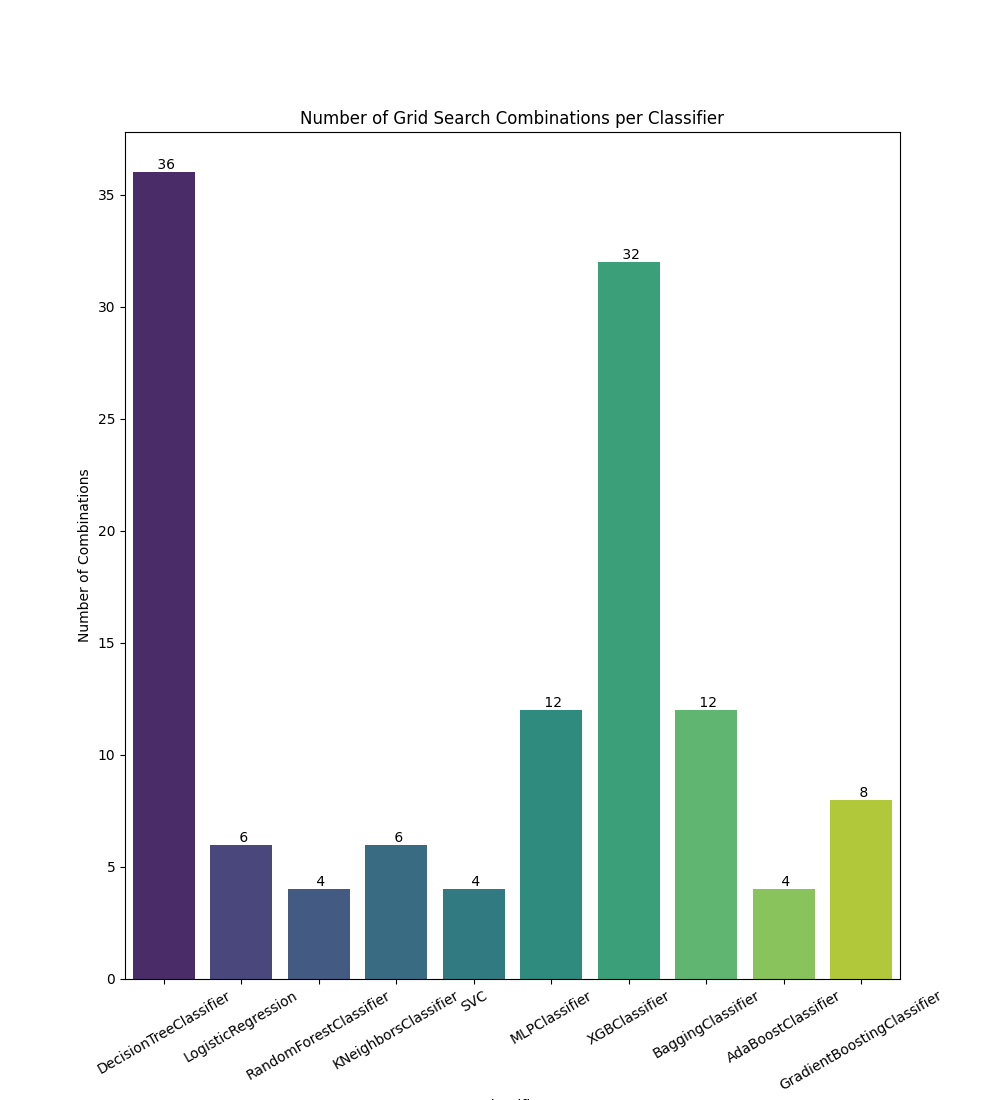
\includegraphics[width=\linewidth]{assets/images/methodology/grid_search_combinations_per_classifier.png}
        \caption{Number of combinations per classifier (124 in total)}
        \label{fig:grid_search_combinations_per_classifier}
    \end{subfigure}
    \hfill
    \begin{subfigure}[b]{0.48\linewidth}
        \centering
        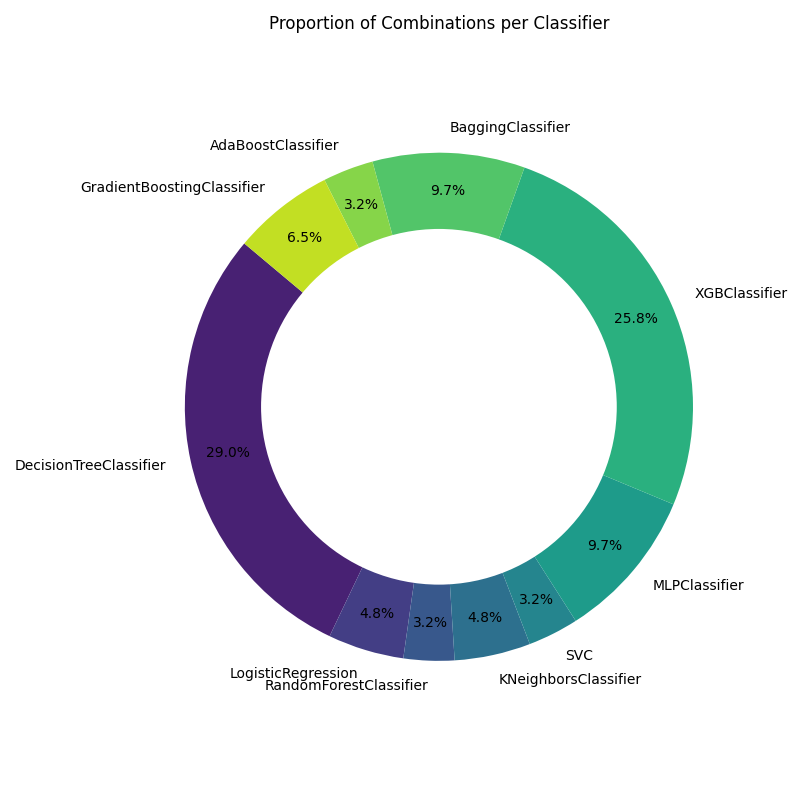
\includegraphics[width=\linewidth]{assets/images/methodology/grid_search_donat.png}
        \caption{Share of combinations per classifier}
        \label{fig:grid_search_donut}
    \end{subfigure}
    \caption{Grid search combinations: (a) absolute number per classifier, (b) share of all combinations.}
    \label{fig:grid_search_analysis}
\end{figure}

% Full-width figure, cropped with trim (left bottom right top)
\begin{figure}[H]
    \centering
    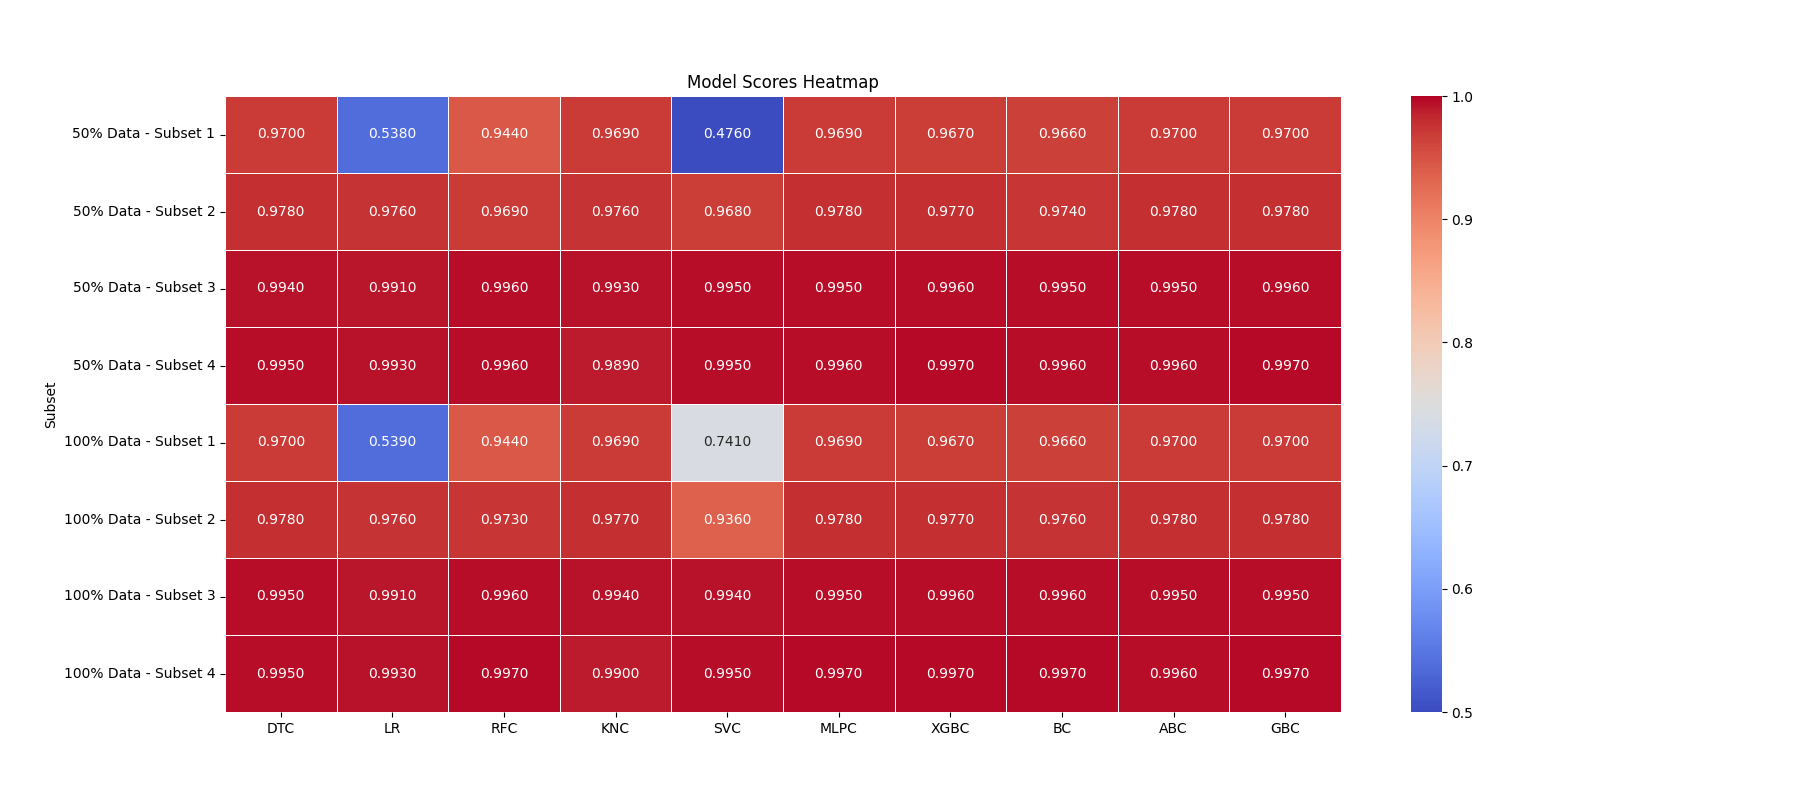
\includegraphics[trim=0cm 0cm 5cm 0cm, clip, width=\linewidth]{assets/images/best_classifier/eval_heatmap.png}
    \caption{Accuracy of each model with its best parameters for two training data sizes (50\,\% and 100\,\%) and
             four feature subsets.}
    \label{fig:eval_heatmap}
\end{figure}
